\documentclass[final,a4paper]{article}
%%% iconv  --from-code=UTF-8 --to-code=ISO-8859-1 x.tex > x_latim.tex
%\usepackage{lucidabr}
%\documentclass[12pt,oneside]{article} % Uma Coluna e lingua portuguesa
%\usepackage[T1]{fontenc}        % Permite digitar os acentos de forma normal
\usepackage[utf8]{inputenc} %% este caso o doc esteja em utf8
%% \usepackage[brazil]{babel}
%\usepackage[latin1]{inputenc}
%\usepackage{epic,eepic} %%,t1enc}

%%% FOR SLIDES DIRECTly
\usepackage[ams]{pdfslide}
\usepackage{graphicx}
%%\overlay{fundo_amarelo.jpg}



%%%%%%%%%%%%%%%%%%%%%%%%%%%%%%%%%
\usepackage{amsmath, amsfonts ,amssymb}
%%%\usepackage{epsfig}   %float,
\usepackage[normalem]{ulem}
\usepackage{hyperref,url}
%\usepackage{pause}
\usepackage{pifont}%,bbding}%%,dingbat} %%% ver manual de simbolos
\usepackage[final]{listings}

%%

\hypersetup{pdftex, colorlinks=true, linkcolor=blue, citecolor=blue, 
filecolor=blue, urlcolor=blue, pdftitle=1, pdfauthor=r4cnr, 
pdfsubject=, pdfkeywords=}
%%% COMMENT UP TO HERE .... 

%%\begin{comment}
\ifx\pdftexversion\undefined
\usepackage[dvips]{graphicx}
\else
\usepackage[pdftex]{graphicx}
\DeclareGraphicsRule{*}{mps}{*}{}
\fi
%%%\end{comment}


%\graphicspath{{./figuresdir1/}{./figuresdir2/}{./figuresdir3/}}
\graphicspath{{/home/claudio/Dropbox/figs_genericas/}{/home/claudio/principal/figs_genericas/}{/home/cc/Dropbox/figs_genericas/}{figuras/}}

%\restylefloat{figure,table}   %%%% obrigat#io... pelo [H]
\overlay{verdinho.pdf}
%%salmao.png}
\pagestyle{title}


%\color{black} 



\begin{document}
%\lstset{language=Prolog}
\lstloadlanguages{Prolog,Haskell,C++}.


\begin{center}
{\huge
Aquecimentols
 da Prova ({\em Warmup})\\
Até Recursividade\\
Joinville, \today 

}
\end{center}



\section{Problema do Caminho na Casa}

\begin{figure}[!htb]
\centering
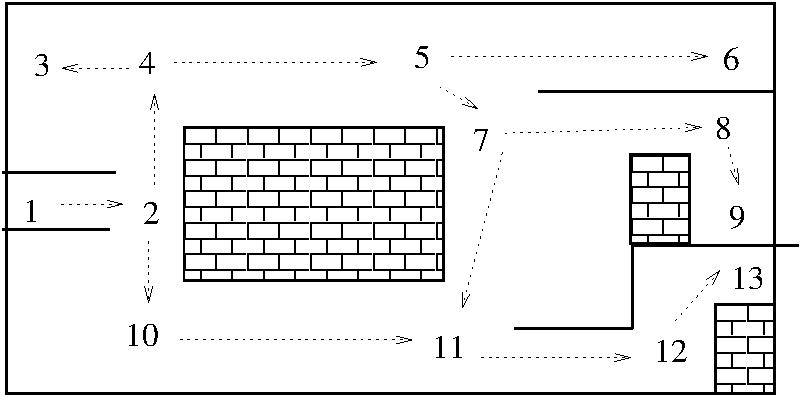
\includegraphics[width=0.8\textwidth , height=0.7\textheight]{casa.pdf}
%%%prolog/scale=0.47
%\label{fig_solutions_covering}
 %\caption{Problemas de Abastecimento -- Alocação}
\end{figure}



\section{Problema de Imprimir o Triângulo}


\begin{figure}[!htb]
\centering
%%\includegraphics[width=0.6\textwidth , height=0.5\textheight]{figuras/trens.png}

\includegraphics[scale=1.3]{triangulo.pdf}
%%%prolog/scale=0.47
%\label{fig_solutions_covering}
 %\caption{Problemas de escalonamento de trens/onibus}
\end{figure}



\end{document}
